\subsection{Technological Background [ASH]}
\blindtext

\subsection{ Sustainability}

\subsubsection{Social [IP]}

One of the long run aims of the Smart Fridge is to reduce food waste by encouraging users to follow habits such as meal planning and consideration of the needless waste of products.
Food waste is one of the key contributing factors to world hunger.
Zero hunger is one of the seventeen UN Sustainable Development Goals [UNGoals].
Growing inequalities is one of the main factors to the undermining of food security worldwide.
Through efforts in trying to reduce food waste, world hunger can be significantly reduced.
Food waste can be broken down in different stages such as harvesting, storage and handling, processing, distribution, retail, and households.
Households have a contribution of approximately 40-50\% of total food waste [FoodWasteStages], which is the largest portion comparing to the rest of the stages of food waste.
There are various reasons behind food waste in households, such as lack of meal planning, and consideration.
A very common scenario is poor planning which occurs when people buy products from the supermarket with the aim of making a specific recipe but also without having a recipe in mind.
In either case, the products might end not being used before their expiration date and hence wasted.
Overbuying is another very common case, where people buy products without considering products that they already have and end up not being able to use them all before their expiration date.  

Another issue that many people face is having poor nutrition, neglecting the importance of eating healthy and nutritious foods.
The Smart Fridge tracks the products contained in the user's fridge and can recommend healthy recipes suggestions, hence promoting a healthier lifestyle.
With Smart Fridge the user can focus on their nutrition which is not very common nowadays.
Additionally, it will be possible to track from anywhere what products they already have and so be reminded of what they own and how they can use it.
Knowing what products they have, allows people to put into consideration what they want to cook, hence be more open to spending time cooking more nutritionally rich foods.
This can be extended to meal planning, depending on the commitment of the user.

\subsubsection{Economic [JG, IP]}

The Smart Fridge allows users to track their groceries and products in their fridge.
This can be done from anywhere using the website, allowing the users to check their products when they are shopping in case they haven't done so before.
This prevents users not only buying products that they might already have, but also consider using the ones they have before buying new ones.
Therefore, grocery shopping can be done more sustainably, while also saving money.
Another aspect of checking the groceries inside the fridge to consider, is that people tend to open and close the fridge door too often, while also leaving it open for long.
This increases the power consumption of the fridge, and so being able to check what is inside the fridge without the need to open and close the door multiple times, the power usage can be decreased, as well as the energy bills of the household.  

According to [The Shocking Amount Of Food U.S.
Households Waste Every Year], the average American household wastes somewhere between 30 to 40\% of their food, which amounts to over 1800 worth of food wasted per household annually or 240 billion in total.
Therefore, one of the goals set out with the Smart Fridge was to design a product that would help households reduce the amount of food they waste.
Each feature of the Smart Fridge was implemented with this goal in mind.

One of the main features of the Smart Fridge is its ability to keep an inventory of what is inside it using a combination of barcode detection software and object recognition.
This is then displayed as a list which can be viewed by the user via a website/app.
This helps the user when making a shopping list as shopping lists help to reduce the purchases of foods that are not really needed.
Additionally, it can also be used by users whilst they are shopping to check if they already have items which they are about to buy.
This prevents the user from buying more food than they can eat, reducing food waste.
This idea is reinforced by [The Shocking Amount Of Food U.S.
Households Waste Every Year], which states that a study observed that households that used shopping lists generally wasted less food than those that did not.

However, [The Shocking Amount Of Food U.S.
Households Waste Every Year] also states that, despite households that used shopping lists wasting less food, even the most frugal household wasted nearly 10\% of their food.
The study conducted in [1] concluded that one of the leading reasons for food waste was food spoiling before the household had the chance to eat it.
Therefore, we have designed a system to automatically detect expiration dates on products, and to remind the user about upcoming expiration dates.
The system works similarly to the barcode detection software in that it uses the camera installed on the door of the fridge to read the expiration dates on products as they enter the fridge.
The goal with this system is to remind the user about expiring food so they can priorities+ the order in which food is consumed based on its expiration date.
These reminders are sent to the user via the website/app.
Additionally, we have used a Hall effect sensor on the door of the fridge to remind the user to keep the door closed.
This will be done via a buzzer and will help to preserve the contents of the fridge so that the expiration dates given by the products are as accurate as possible.  

The previous methods for reducing food waste focus on minimizing the amount of food that is thrown away.
However, this next feature focusses on maximising the amount of food used, which is the another approach to minimising food waste.
We have implemented a feature on the website/app which will recommend recipes to the user based on the contents of the fridge.
The study discussed in [1] mentions that households with healthier diets generally wasted more food.
This is due to an increased use of fruit and vegetables which spoil sooner than other foods.
Therefore, our goal with this feature was to ensure that food bought by the user is used efficiently.
The idea is that, as the recommended recipes are based on the contents of the fridge, the user will stick to the ingredients they already have rather than continuing to buy more, helping them to use as much of the food that they have already bought as possible.
Therefore, less food will be wasted and the user will save money on having to replace the wasted food.

\subsubsection{Environmental [IP]} 
Preventing food waste can alleviate the negative impact it has on the environment.
Most people that overbuy and don't meal plan end up wasting a lot of the products they have bought as these products have either expired and cannot be used.
All food waste can have a significant contribution to global warming.
Food waste breaks down in landfills and decomposes into methane that is released in the atmosphere.
Methane is one of the key greenhouse gases contributing to global warming [foodwaste].
Therefore, having a system that allows tracking and reducing the waste of products, can have a positive effect in the minimisation of food waste.
Additionally, as forementioned the tracking of products through a website, can reduce the power usage of the fridge as the user minimises the time, they have the fridge door open.
The UN Sustainability Goals aimed to be approached through the Smart Fridge are the following:

\begin{itemize}
    \item Goal 2 - Zero Hunger
    \item Goal 3 - Good Health and Well-being
    \item Goal 8 - Decent 	Work and Economic Growth
    \item Goal 12 - Responsible Consumption and Production
    \item Goal 13 - Climate Action 
\end{itemize}

\subsection{System Overview [IB]}
The objective of the overall system is to autonomously track the inventory of a fridge.
Our approach to solve this objective was to split the system into several sub systems.
There are 4 components connected to the ESP32 microcontroller: the HX711 load cell measures the weight of the contents of the fridge and needs between 3.3V and 5V to operate, a HAL sensor requires 2.8-6V of power and is used to detect weather the fridge door is open, a 5V LED strip to light up the fridge and a buzzer that sounds when the fridge has been open too long.
The direction of the item is quantified by calculating the change in weight.
This value is packaged in a JSON packet with the ON/OFF state of the fridge door and the alarm state and sent to the Raspberry Pi via UART serial communication.
The hardware is powered by a 9V barrel jack and is stepped down by a switch mode power supply to 3.3V and 5V.
A 5V USB web camera is connected to the PI and captures the item as it enters the fridge.
OpenCV is used to detect what item is entering the fridge.
The inventory information and the direction are then sent to a PostgreSQL database using GraphQL communication.
Depending on the item's direction, the item will be added or removed from the database.
This database acts as a backend for the products website/app.

\begin{figure}[H]        
    \centering
    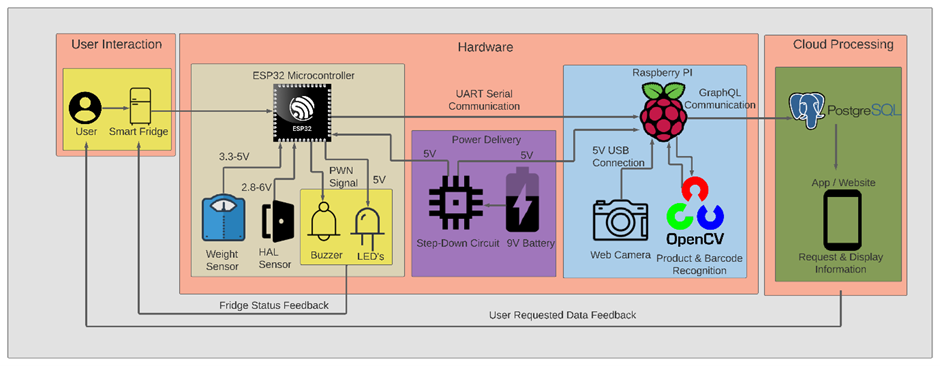
\includegraphics[width=1\textwidth]{Chapter 2/SystemOverview.png}
    \caption{System Overview Block Diagram}
    \label{fig:blockdia}
\end{figure} 

The project can be split into 3 main groups: the microprocessor group who will design the hardware which will collect the data, the Raspberry Pi group who will use OpenCV to detect the item and the cloud processing team who will deal with the server and website side of the design.
Within each group the tasks can be split between each member.
For example, in the microprocessor team, each member can be assigned to a different component and in the cloud processing team one member can focus on the front-end design and the other on the back end.
By splitting the project into smaller objectives, work can be completed independently and in parallel and the number dependencies between members can be reduced.
This will make the project run much more efficiently.
The individual teams will however need to communicate when planning on how to integrate the work together.
The sub systems and their dependencies have been outlined in table 'XXXXXXXXXXXXXX'.

\subsection{Dependency Table [IB]}
% Please add the following required packages to your document preamble:
% \usepackage{longtable}
% Note: It may be necessary to compile the document several times to get a multi-page table to line up properly
\small
\begin{longtable}[c]{|l|l|l|}
    \caption{Member Contributions and Goals}
    \label{tab:conrib}\\
    \hline
    Team Member &
      Contributions &
      Aims \\ \hline
    \endfirsthead
    %
    \endhead
    %
    Isaac Baglin - IB &
      \begin{tabular}[c]{@{}l@{}}Design Brief: Overview, SAGE assessment\\ form \\  \\ Project Work: Weight Sensor, Esp Camera\\ Module, Buzzer and Debugging  \\  \\ Final Report: System Overview, Smart\\ Fridge Dependency Table, Smart Fridge\\ MOSCOW Diagram, SWOT Analysis, Client\\ Brief Requirement Checklist, Phase Diagram\\ and Description, Weight Sensor Development,\\ Esp32-Wrover Dec-Board Camera\\ Development, Buzzer Development.\end{tabular} &
      \begin{tabular}[c]{@{}l@{}}My goal for this project was to develop\\ skills in systems engineering. To do this,\\ I put myself on the microprocessor team\\ so that I could plan, design, and integrate\\ subsystems.\end{tabular} \\ \hline
    \begin{tabular}[c]{@{}l@{}}Jamie \\ Gomez - JG\end{tabular} &
      \begin{tabular}[c]{@{}l@{}}Design Brief:  Project Management \\  \\ Project Work: Barcode detection, box design \\  \\ Final Report: Economic benefits, Barcode\\ detection, box design prototype 1\end{tabular} &
      \begin{tabular}[c]{@{}l@{}}My aim for this project was to develop my\\ teamwork skills. This was achieved mainly\\ when working on the box design where, \\ throughout the project, it was necessary\\ to listen to the requirements of each team\\ to design a box that best fitted everyone’s\\ needs. \\  \\ With barcode detection my aim was to find\\ and test suitable algorithms in order to\\ select the best one for this product.\end{tabular} \\ \hline
    \begin{tabular}[c]{@{}l@{}}Hamzah \\ Hasnain - HH\end{tabular} &
      \begin{tabular}[c]{@{}l@{}}Design Brief: Sustainability \\  \\ Project Work: Website Creation,\\ LEDs \\  \\ Final Report: Website, LEDs,\\ Sustainability, Circular Economy\end{tabular} &
      \begin{tabular}[c]{@{}l@{}}My goals for this project were to develop my\\ skills, specifically my skills in software and\\ programming. I took responsibility of creating\\ a website. Since I had not previously created\\ a website, there was a lot to learn. Learn how\\ web applications and hardware are integrated \\ I also wanted to gain experience with\\ programming hardware and understand\\ different methods of achieving a software-\\ hardware solution.\end{tabular} \\ \hline
    \begin{tabular}[c]{@{}l@{}}Ioanna \\ Papanikolaou - IP\end{tabular} &
      \begin{tabular}[c]{@{}l@{}}Design Brief: Technical Outline,Sustainability\\ discussion \\  \\ Project Work: \\ Object detection, character recognition,\\ model training  \\  \\ Final Report: Social, Economic and\\ Environmental impacts discussion, Software\\ Section\end{tabular} &
      \begin{tabular}[c]{@{}l@{}}My goals for this project were to develop my\\ software and team working skills. I was in the\\ software team with the aim of developing a \\ model that would classify the objects, acting\\ as an object recognition system. It was also\\ important for me to improve my teamwork\\ skills especially in software as so far I have\\ been mainly working on my own.\end{tabular} \\ \hline
    Yohan John - YJ &
      \begin{tabular}[c]{@{}l@{}}Design Brief: Technical Outline \\  \\ Project Work:  Architect the firmware code,\\ Hal Sensor Integration, Software – Timer\\ for buzzer feature. Comms between\\ raspberry pi and esp32, Debugging.\\ Designed Prototype 1. Designed and\\ built Prototype2 \\  \\ Final Report:  Hardware Outline, Firmware\\ Code, and Box Design and Build Prototyp2\end{tabular} &
      \begin{tabular}[c]{@{}l@{}}My goals for the group project included\\ developing my skills in both the technical\\ and management side. I wanted to take\\ more responsibility for organising the team\\ and architecting the software for the\\ microcontroller. I also aim to be an active\\ team member and contribute resources\\ when required.\end{tabular} \\ \hline
    \begin{tabular}[c]{@{}l@{}}Alexandre\\ Symeonidis-Herzig - ASH\end{tabular} &
      \begin{tabular}[c]{@{}l@{}}Design Brief: Appendices, Latex Compiling,\\ Revising document.  \\  \\ Project Work: Designed Pi Hat (PCB), Power\\ distribution board, Developed React Native\\ App and Created Supabase DB. \\  \\ Final Report: Tech background, Pi Hat PCB\\ design, Power distribution, Mobile App,\\ Supabase DB, Raspberry Pi Refactor\\ as well as compiling in LaTeX, editing\\ the document and formatting citations.\end{tabular} &
      \begin{tabular}[c]{@{}l@{}}To learn about and integrate all the \\ components for an app, from databases\\ and hosting to UI design and functionality.  \\   \\ Also, to focus on the learning the planning\\ required to get a more complicated project\\ from idea to prototype especially with a\\ larger team.\end{tabular} \\ \hline
    Alfie Walding - AW &
      \begin{tabular}[c]{@{}l@{}}Design Brief: Gantt Chart, Project\\ Management, Compiling and Revising\\ document.  \\  \\ Project Work: Raspberry Pi installation\\ and setup, Raspberry Pi camera setup,\\ Barcode detection development,\\ Raspberry Pi Serial communication,\\ Barcode detection integration, OCR code\\ integration, Product detection integration,\\ Supabase database integration and\\ Raspberry Pi refactoring. \\  \\ Final Report: Introduction, Pi Overview,\\ Pi camera, Pi serial input, Pi integration,\\ Pi refactoring as well as compiling and\\ revising the document.\end{tabular} &
      \begin{tabular}[c]{@{}l@{}}To successfully integrate and combine the \\ character, product, and barcode detection\\ code, onto the Raspberry Pi. The code should\\ function together flawlessly with compatibility\\ issues being fixed and required modules \\ imported. \\  \\ To receive data from the ESP and process it \\ into a format that can be communicated to \\ the database.  \\  \\ To successfully detect barcodes in images so\\ they can be sent to the database. \\  \\ To develop skills and knowledge of the\\ Raspberry Pi and the Linux operating system.\end{tabular} \\ \hline
\end{longtable}

\subsection{MOSCOW Diagram [IB]}
% Please add the following required packages to your document preamble:
% \usepackage{longtable}
% Note: It may be necessary to compile the document several times to get a multi-page table to line up properly
\small
\begin{longtable}[c]{|l|l|l|}
    \caption{Member Contributions and Goals}
    \label{tab:conrib}\\
    \hline
    Team Member &
      Contributions &
      Aims \\ \hline
    \endfirsthead
    %
    \endhead
    %
    Isaac Baglin - IB &
      \begin{tabular}[c]{@{}l@{}}Design Brief: Overview, SAGE assessment\\ form \\  \\ Project Work: Weight Sensor, Esp Camera\\ Module, Buzzer and Debugging  \\  \\ Final Report: System Overview, Smart\\ Fridge Dependency Table, Smart Fridge\\ MOSCOW Diagram, SWOT Analysis, Client\\ Brief Requirement Checklist, Phase Diagram\\ and Description, Weight Sensor Development,\\ Esp32-Wrover Dec-Board Camera\\ Development, Buzzer Development.\end{tabular} &
      \begin{tabular}[c]{@{}l@{}}My goal for this project was to develop\\ skills in systems engineering. To do this,\\ I put myself on the microprocessor team\\ so that I could plan, design, and integrate\\ subsystems.\end{tabular} \\ \hline
    \begin{tabular}[c]{@{}l@{}}Jamie \\ Gomez - JG\end{tabular} &
      \begin{tabular}[c]{@{}l@{}}Design Brief:  Project Management \\  \\ Project Work: Barcode detection, box design \\  \\ Final Report: Economic benefits, Barcode\\ detection, box design prototype 1\end{tabular} &
      \begin{tabular}[c]{@{}l@{}}My aim for this project was to develop my\\ teamwork skills. This was achieved mainly\\ when working on the box design where, \\ throughout the project, it was necessary\\ to listen to the requirements of each team\\ to design a box that best fitted everyone’s\\ needs. \\  \\ With barcode detection my aim was to find\\ and test suitable algorithms in order to\\ select the best one for this product.\end{tabular} \\ \hline
    \begin{tabular}[c]{@{}l@{}}Hamzah \\ Hasnain - HH\end{tabular} &
      \begin{tabular}[c]{@{}l@{}}Design Brief: Sustainability \\  \\ Project Work: Website Creation,\\ LEDs \\  \\ Final Report: Website, LEDs,\\ Sustainability, Circular Economy\end{tabular} &
      \begin{tabular}[c]{@{}l@{}}My goals for this project were to develop my\\ skills, specifically my skills in software and\\ programming. I took responsibility of creating\\ a website. Since I had not previously created\\ a website, there was a lot to learn. Learn how\\ web applications and hardware are integrated \\ I also wanted to gain experience with\\ programming hardware and understand\\ different methods of achieving a software-\\ hardware solution.\end{tabular} \\ \hline
    \begin{tabular}[c]{@{}l@{}}Ioanna \\ Papanikolaou - IP\end{tabular} &
      \begin{tabular}[c]{@{}l@{}}Design Brief: Technical Outline,Sustainability\\ discussion \\  \\ Project Work: \\ Object detection, character recognition,\\ model training  \\  \\ Final Report: Social, Economic and\\ Environmental impacts discussion, Software\\ Section\end{tabular} &
      \begin{tabular}[c]{@{}l@{}}My goals for this project were to develop my\\ software and team working skills. I was in the\\ software team with the aim of developing a \\ model that would classify the objects, acting\\ as an object recognition system. It was also\\ important for me to improve my teamwork\\ skills especially in software as so far I have\\ been mainly working on my own.\end{tabular} \\ \hline
    Yohan John - YJ &
      \begin{tabular}[c]{@{}l@{}}Design Brief: Technical Outline \\  \\ Project Work:  Architect the firmware code,\\ Hal Sensor Integration, Software – Timer\\ for buzzer feature. Comms between\\ raspberry pi and esp32, Debugging.\\ Designed Prototype 1. Designed and\\ built Prototype2 \\  \\ Final Report:  Hardware Outline, Firmware\\ Code, and Box Design and Build Prototyp2\end{tabular} &
      \begin{tabular}[c]{@{}l@{}}My goals for the group project included\\ developing my skills in both the technical\\ and management side. I wanted to take\\ more responsibility for organising the team\\ and architecting the software for the\\ microcontroller. I also aim to be an active\\ team member and contribute resources\\ when required.\end{tabular} \\ \hline
    \begin{tabular}[c]{@{}l@{}}Alexandre\\ Symeonidis-Herzig - ASH\end{tabular} &
      \begin{tabular}[c]{@{}l@{}}Design Brief: Appendices, Latex Compiling,\\ Revising document.  \\  \\ Project Work: Designed Pi Hat (PCB), Power\\ distribution board, Developed React Native\\ App and Created Supabase DB. \\  \\ Final Report: Tech background, Pi Hat PCB\\ design, Power distribution, Mobile App,\\ Supabase DB, Raspberry Pi Refactor\\ as well as compiling in LaTeX, editing\\ the document and formatting citations.\end{tabular} &
      \begin{tabular}[c]{@{}l@{}}To learn about and integrate all the \\ components for an app, from databases\\ and hosting to UI design and functionality.  \\   \\ Also, to focus on the learning the planning\\ required to get a more complicated project\\ from idea to prototype especially with a\\ larger team.\end{tabular} \\ \hline
    Alfie Walding - AW &
      \begin{tabular}[c]{@{}l@{}}Design Brief: Gantt Chart, Project\\ Management, Compiling and Revising\\ document.  \\  \\ Project Work: Raspberry Pi installation\\ and setup, Raspberry Pi camera setup,\\ Barcode detection development,\\ Raspberry Pi Serial communication,\\ Barcode detection integration, OCR code\\ integration, Product detection integration,\\ Supabase database integration and\\ Raspberry Pi refactoring. \\  \\ Final Report: Introduction, Pi Overview,\\ Pi camera, Pi serial input, Pi integration,\\ Pi refactoring as well as compiling and\\ revising the document.\end{tabular} &
      \begin{tabular}[c]{@{}l@{}}To successfully integrate and combine the \\ character, product, and barcode detection\\ code, onto the Raspberry Pi. The code should\\ function together flawlessly with compatibility\\ issues being fixed and required modules \\ imported. \\  \\ To receive data from the ESP and process it \\ into a format that can be communicated to \\ the database.  \\  \\ To successfully detect barcodes in images so\\ they can be sent to the database. \\  \\ To develop skills and knowledge of the\\ Raspberry Pi and the Linux operating system.\end{tabular} \\ \hline
\end{longtable}

\subsection{SWOT Analysis [IB]}
% Please add the following required packages to your document preamble:
% \usepackage{longtable}
% Note: It may be necessary to compile the document several times to get a multi-page table to line up properly
\small
\begin{longtable}[c]{|l|l|l|}
    \caption{Member Contributions and Goals}
    \label{tab:conrib}\\
    \hline
    Team Member &
      Contributions &
      Aims \\ \hline
    \endfirsthead
    %
    \endhead
    %
    Isaac Baglin - IB &
      \begin{tabular}[c]{@{}l@{}}Design Brief: Overview, SAGE assessment\\ form \\  \\ Project Work: Weight Sensor, Esp Camera\\ Module, Buzzer and Debugging  \\  \\ Final Report: System Overview, Smart\\ Fridge Dependency Table, Smart Fridge\\ MOSCOW Diagram, SWOT Analysis, Client\\ Brief Requirement Checklist, Phase Diagram\\ and Description, Weight Sensor Development,\\ Esp32-Wrover Dec-Board Camera\\ Development, Buzzer Development.\end{tabular} &
      \begin{tabular}[c]{@{}l@{}}My goal for this project was to develop\\ skills in systems engineering. To do this,\\ I put myself on the microprocessor team\\ so that I could plan, design, and integrate\\ subsystems.\end{tabular} \\ \hline
    \begin{tabular}[c]{@{}l@{}}Jamie \\ Gomez - JG\end{tabular} &
      \begin{tabular}[c]{@{}l@{}}Design Brief:  Project Management \\  \\ Project Work: Barcode detection, box design \\  \\ Final Report: Economic benefits, Barcode\\ detection, box design prototype 1\end{tabular} &
      \begin{tabular}[c]{@{}l@{}}My aim for this project was to develop my\\ teamwork skills. This was achieved mainly\\ when working on the box design where, \\ throughout the project, it was necessary\\ to listen to the requirements of each team\\ to design a box that best fitted everyone’s\\ needs. \\  \\ With barcode detection my aim was to find\\ and test suitable algorithms in order to\\ select the best one for this product.\end{tabular} \\ \hline
    \begin{tabular}[c]{@{}l@{}}Hamzah \\ Hasnain - HH\end{tabular} &
      \begin{tabular}[c]{@{}l@{}}Design Brief: Sustainability \\  \\ Project Work: Website Creation,\\ LEDs \\  \\ Final Report: Website, LEDs,\\ Sustainability, Circular Economy\end{tabular} &
      \begin{tabular}[c]{@{}l@{}}My goals for this project were to develop my\\ skills, specifically my skills in software and\\ programming. I took responsibility of creating\\ a website. Since I had not previously created\\ a website, there was a lot to learn. Learn how\\ web applications and hardware are integrated \\ I also wanted to gain experience with\\ programming hardware and understand\\ different methods of achieving a software-\\ hardware solution.\end{tabular} \\ \hline
    \begin{tabular}[c]{@{}l@{}}Ioanna \\ Papanikolaou - IP\end{tabular} &
      \begin{tabular}[c]{@{}l@{}}Design Brief: Technical Outline,Sustainability\\ discussion \\  \\ Project Work: \\ Object detection, character recognition,\\ model training  \\  \\ Final Report: Social, Economic and\\ Environmental impacts discussion, Software\\ Section\end{tabular} &
      \begin{tabular}[c]{@{}l@{}}My goals for this project were to develop my\\ software and team working skills. I was in the\\ software team with the aim of developing a \\ model that would classify the objects, acting\\ as an object recognition system. It was also\\ important for me to improve my teamwork\\ skills especially in software as so far I have\\ been mainly working on my own.\end{tabular} \\ \hline
    Yohan John - YJ &
      \begin{tabular}[c]{@{}l@{}}Design Brief: Technical Outline \\  \\ Project Work:  Architect the firmware code,\\ Hal Sensor Integration, Software – Timer\\ for buzzer feature. Comms between\\ raspberry pi and esp32, Debugging.\\ Designed Prototype 1. Designed and\\ built Prototype2 \\  \\ Final Report:  Hardware Outline, Firmware\\ Code, and Box Design and Build Prototyp2\end{tabular} &
      \begin{tabular}[c]{@{}l@{}}My goals for the group project included\\ developing my skills in both the technical\\ and management side. I wanted to take\\ more responsibility for organising the team\\ and architecting the software for the\\ microcontroller. I also aim to be an active\\ team member and contribute resources\\ when required.\end{tabular} \\ \hline
    \begin{tabular}[c]{@{}l@{}}Alexandre\\ Symeonidis-Herzig - ASH\end{tabular} &
      \begin{tabular}[c]{@{}l@{}}Design Brief: Appendices, Latex Compiling,\\ Revising document.  \\  \\ Project Work: Designed Pi Hat (PCB), Power\\ distribution board, Developed React Native\\ App and Created Supabase DB. \\  \\ Final Report: Tech background, Pi Hat PCB\\ design, Power distribution, Mobile App,\\ Supabase DB, Raspberry Pi Refactor\\ as well as compiling in LaTeX, editing\\ the document and formatting citations.\end{tabular} &
      \begin{tabular}[c]{@{}l@{}}To learn about and integrate all the \\ components for an app, from databases\\ and hosting to UI design and functionality.  \\   \\ Also, to focus on the learning the planning\\ required to get a more complicated project\\ from idea to prototype especially with a\\ larger team.\end{tabular} \\ \hline
    Alfie Walding - AW &
      \begin{tabular}[c]{@{}l@{}}Design Brief: Gantt Chart, Project\\ Management, Compiling and Revising\\ document.  \\  \\ Project Work: Raspberry Pi installation\\ and setup, Raspberry Pi camera setup,\\ Barcode detection development,\\ Raspberry Pi Serial communication,\\ Barcode detection integration, OCR code\\ integration, Product detection integration,\\ Supabase database integration and\\ Raspberry Pi refactoring. \\  \\ Final Report: Introduction, Pi Overview,\\ Pi camera, Pi serial input, Pi integration,\\ Pi refactoring as well as compiling and\\ revising the document.\end{tabular} &
      \begin{tabular}[c]{@{}l@{}}To successfully integrate and combine the \\ character, product, and barcode detection\\ code, onto the Raspberry Pi. The code should\\ function together flawlessly with compatibility\\ issues being fixed and required modules \\ imported. \\  \\ To receive data from the ESP and process it \\ into a format that can be communicated to \\ the database.  \\  \\ To successfully detect barcodes in images so\\ they can be sent to the database. \\  \\ To develop skills and knowledge of the\\ Raspberry Pi and the Linux operating system.\end{tabular} \\ \hline
\end{longtable}

\subsection{Client Requirements [IB]}
% Please add the following required packages to your document preamble:
% \usepackage{longtable}
% Note: It may be necessary to compile the document several times to get a multi-page table to line up properly
\small
\begin{longtable}[c]{|l|l|l|}
    \caption{Member Contributions and Goals}
    \label{tab:conrib}\\
    \hline
    Team Member &
      Contributions &
      Aims \\ \hline
    \endfirsthead
    %
    \endhead
    %
    Isaac Baglin - IB &
      \begin{tabular}[c]{@{}l@{}}Design Brief: Overview, SAGE assessment\\ form \\  \\ Project Work: Weight Sensor, Esp Camera\\ Module, Buzzer and Debugging  \\  \\ Final Report: System Overview, Smart\\ Fridge Dependency Table, Smart Fridge\\ MOSCOW Diagram, SWOT Analysis, Client\\ Brief Requirement Checklist, Phase Diagram\\ and Description, Weight Sensor Development,\\ Esp32-Wrover Dec-Board Camera\\ Development, Buzzer Development.\end{tabular} &
      \begin{tabular}[c]{@{}l@{}}My goal for this project was to develop\\ skills in systems engineering. To do this,\\ I put myself on the microprocessor team\\ so that I could plan, design, and integrate\\ subsystems.\end{tabular} \\ \hline
    \begin{tabular}[c]{@{}l@{}}Jamie \\ Gomez - JG\end{tabular} &
      \begin{tabular}[c]{@{}l@{}}Design Brief:  Project Management \\  \\ Project Work: Barcode detection, box design \\  \\ Final Report: Economic benefits, Barcode\\ detection, box design prototype 1\end{tabular} &
      \begin{tabular}[c]{@{}l@{}}My aim for this project was to develop my\\ teamwork skills. This was achieved mainly\\ when working on the box design where, \\ throughout the project, it was necessary\\ to listen to the requirements of each team\\ to design a box that best fitted everyone’s\\ needs. \\  \\ With barcode detection my aim was to find\\ and test suitable algorithms in order to\\ select the best one for this product.\end{tabular} \\ \hline
    \begin{tabular}[c]{@{}l@{}}Hamzah \\ Hasnain - HH\end{tabular} &
      \begin{tabular}[c]{@{}l@{}}Design Brief: Sustainability \\  \\ Project Work: Website Creation,\\ LEDs \\  \\ Final Report: Website, LEDs,\\ Sustainability, Circular Economy\end{tabular} &
      \begin{tabular}[c]{@{}l@{}}My goals for this project were to develop my\\ skills, specifically my skills in software and\\ programming. I took responsibility of creating\\ a website. Since I had not previously created\\ a website, there was a lot to learn. Learn how\\ web applications and hardware are integrated \\ I also wanted to gain experience with\\ programming hardware and understand\\ different methods of achieving a software-\\ hardware solution.\end{tabular} \\ \hline
    \begin{tabular}[c]{@{}l@{}}Ioanna \\ Papanikolaou - IP\end{tabular} &
      \begin{tabular}[c]{@{}l@{}}Design Brief: Technical Outline,Sustainability\\ discussion \\  \\ Project Work: \\ Object detection, character recognition,\\ model training  \\  \\ Final Report: Social, Economic and\\ Environmental impacts discussion, Software\\ Section\end{tabular} &
      \begin{tabular}[c]{@{}l@{}}My goals for this project were to develop my\\ software and team working skills. I was in the\\ software team with the aim of developing a \\ model that would classify the objects, acting\\ as an object recognition system. It was also\\ important for me to improve my teamwork\\ skills especially in software as so far I have\\ been mainly working on my own.\end{tabular} \\ \hline
    Yohan John - YJ &
      \begin{tabular}[c]{@{}l@{}}Design Brief: Technical Outline \\  \\ Project Work:  Architect the firmware code,\\ Hal Sensor Integration, Software – Timer\\ for buzzer feature. Comms between\\ raspberry pi and esp32, Debugging.\\ Designed Prototype 1. Designed and\\ built Prototype2 \\  \\ Final Report:  Hardware Outline, Firmware\\ Code, and Box Design and Build Prototyp2\end{tabular} &
      \begin{tabular}[c]{@{}l@{}}My goals for the group project included\\ developing my skills in both the technical\\ and management side. I wanted to take\\ more responsibility for organising the team\\ and architecting the software for the\\ microcontroller. I also aim to be an active\\ team member and contribute resources\\ when required.\end{tabular} \\ \hline
    \begin{tabular}[c]{@{}l@{}}Alexandre\\ Symeonidis-Herzig - ASH\end{tabular} &
      \begin{tabular}[c]{@{}l@{}}Design Brief: Appendices, Latex Compiling,\\ Revising document.  \\  \\ Project Work: Designed Pi Hat (PCB), Power\\ distribution board, Developed React Native\\ App and Created Supabase DB. \\  \\ Final Report: Tech background, Pi Hat PCB\\ design, Power distribution, Mobile App,\\ Supabase DB, Raspberry Pi Refactor\\ as well as compiling in LaTeX, editing\\ the document and formatting citations.\end{tabular} &
      \begin{tabular}[c]{@{}l@{}}To learn about and integrate all the \\ components for an app, from databases\\ and hosting to UI design and functionality.  \\   \\ Also, to focus on the learning the planning\\ required to get a more complicated project\\ from idea to prototype especially with a\\ larger team.\end{tabular} \\ \hline
    Alfie Walding - AW &
      \begin{tabular}[c]{@{}l@{}}Design Brief: Gantt Chart, Project\\ Management, Compiling and Revising\\ document.  \\  \\ Project Work: Raspberry Pi installation\\ and setup, Raspberry Pi camera setup,\\ Barcode detection development,\\ Raspberry Pi Serial communication,\\ Barcode detection integration, OCR code\\ integration, Product detection integration,\\ Supabase database integration and\\ Raspberry Pi refactoring. \\  \\ Final Report: Introduction, Pi Overview,\\ Pi camera, Pi serial input, Pi integration,\\ Pi refactoring as well as compiling and\\ revising the document.\end{tabular} &
      \begin{tabular}[c]{@{}l@{}}To successfully integrate and combine the \\ character, product, and barcode detection\\ code, onto the Raspberry Pi. The code should\\ function together flawlessly with compatibility\\ issues being fixed and required modules \\ imported. \\  \\ To receive data from the ESP and process it \\ into a format that can be communicated to \\ the database.  \\  \\ To successfully detect barcodes in images so\\ they can be sent to the database. \\  \\ To develop skills and knowledge of the\\ Raspberry Pi and the Linux operating system.\end{tabular} \\ \hline
\end{longtable}

\subsection{Phase Diagram [IB]}

\begin{figure}[H]        
    \centering
    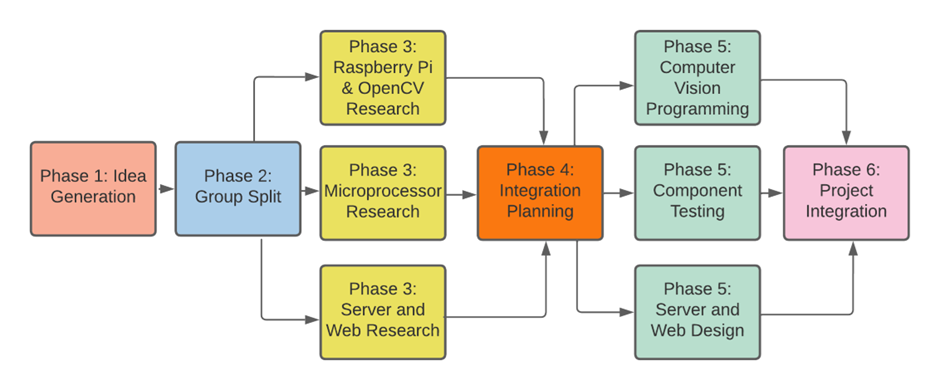
\includegraphics[width=1\textwidth]{Chapter 2/PhaseDiagram.png}
    \caption{Phase Diagram}
    \label{fig:phasediag}
\end{figure} 

The first phase of the project was to generate ideas for the project which followed the specification and vote on which idea to put forward.
Phase 2 is when the group discusses the individual members strengths and weaknesses and decides who is best suited to each team.
Phase 3 is the research phase, and it involves looking into what software and components could be used whilst considering their feasibility.

At the end of this phase a plan should be formed to start designing and testing the tasks of each group as well as ordering the required parts.
Phase 4 is aimed at coming together as a group and forming a plan to integrate the individual teams work together.
This includes discussions of dependencies that each sub team have on each other.
Phase 5 is when the individual teams build and test their work and phase 6 is when the work of the 3 teams is integrated together.